\section{Results}
\label{sec:results}

\begin{figure}
\centering
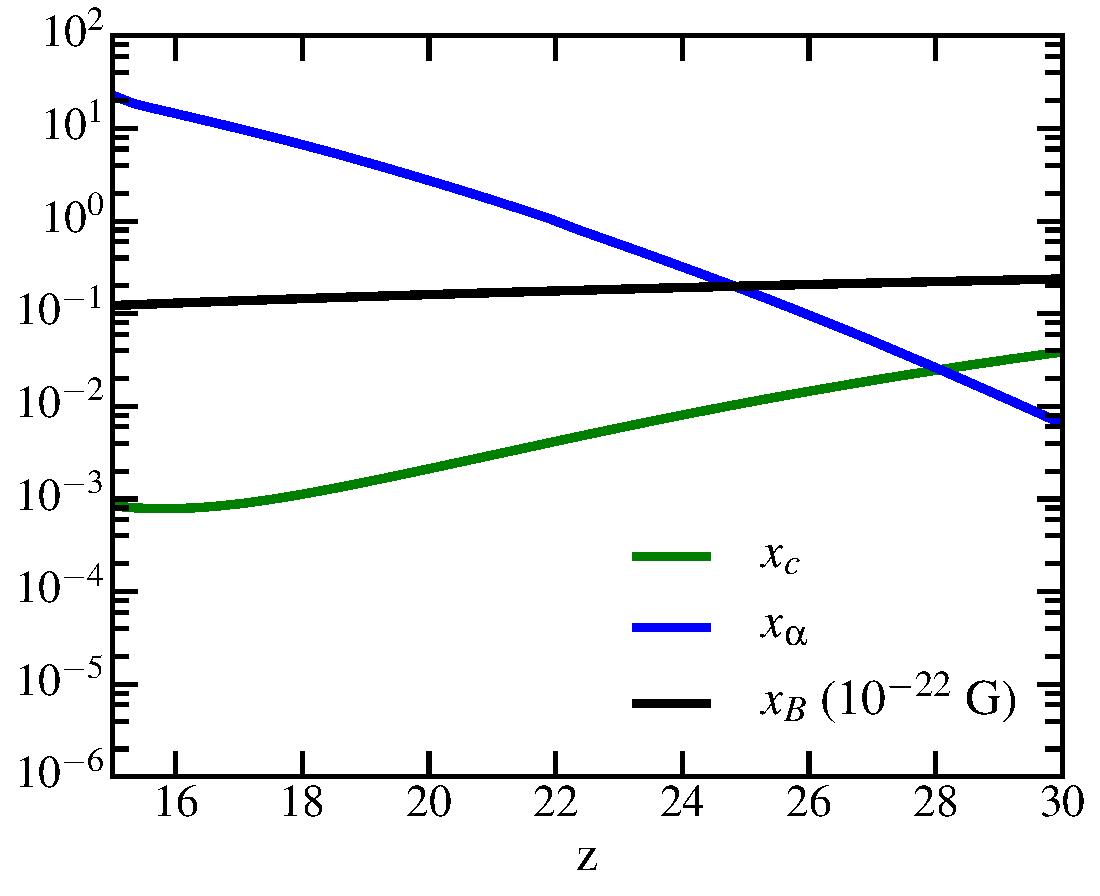
\includegraphics[width=.35\textwidth,keepaspectratio=true]{xs.pdf}
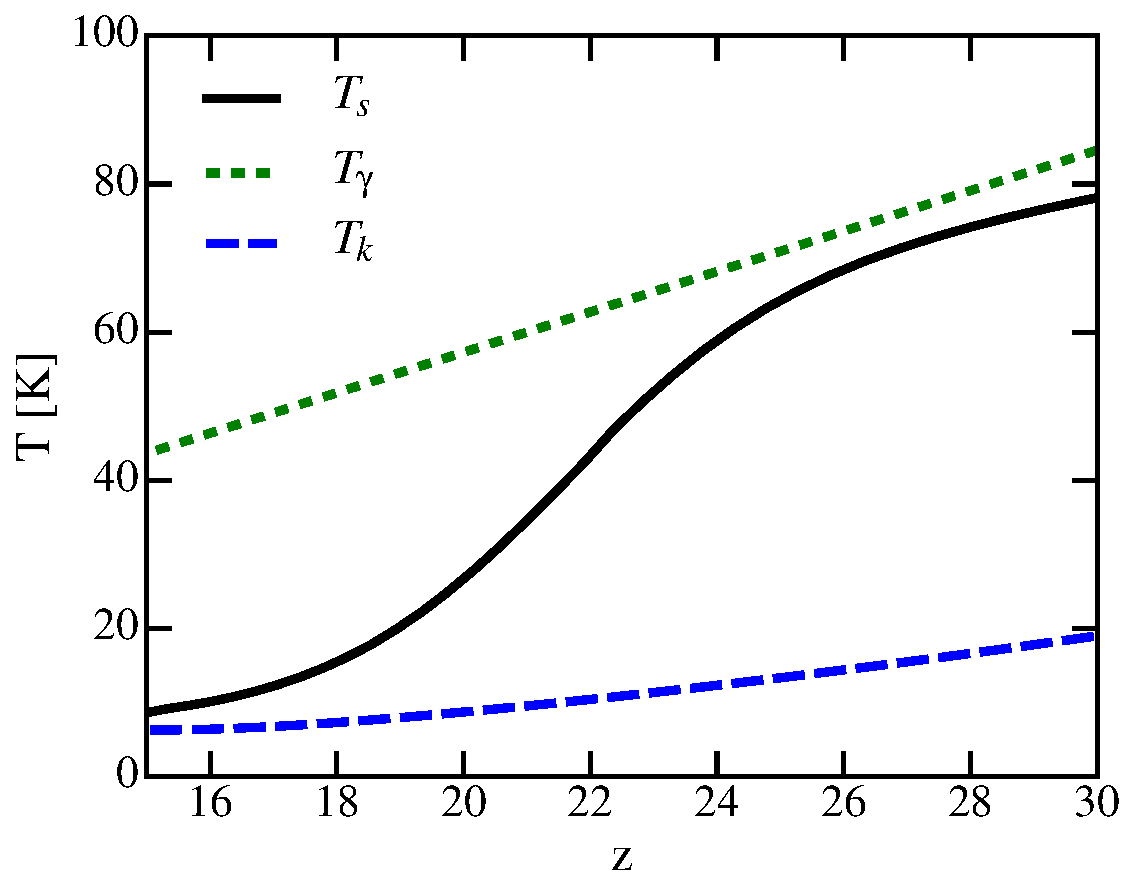
\includegraphics[width=.35\textwidth,keepaspectratio=true]{Ts.pdf}
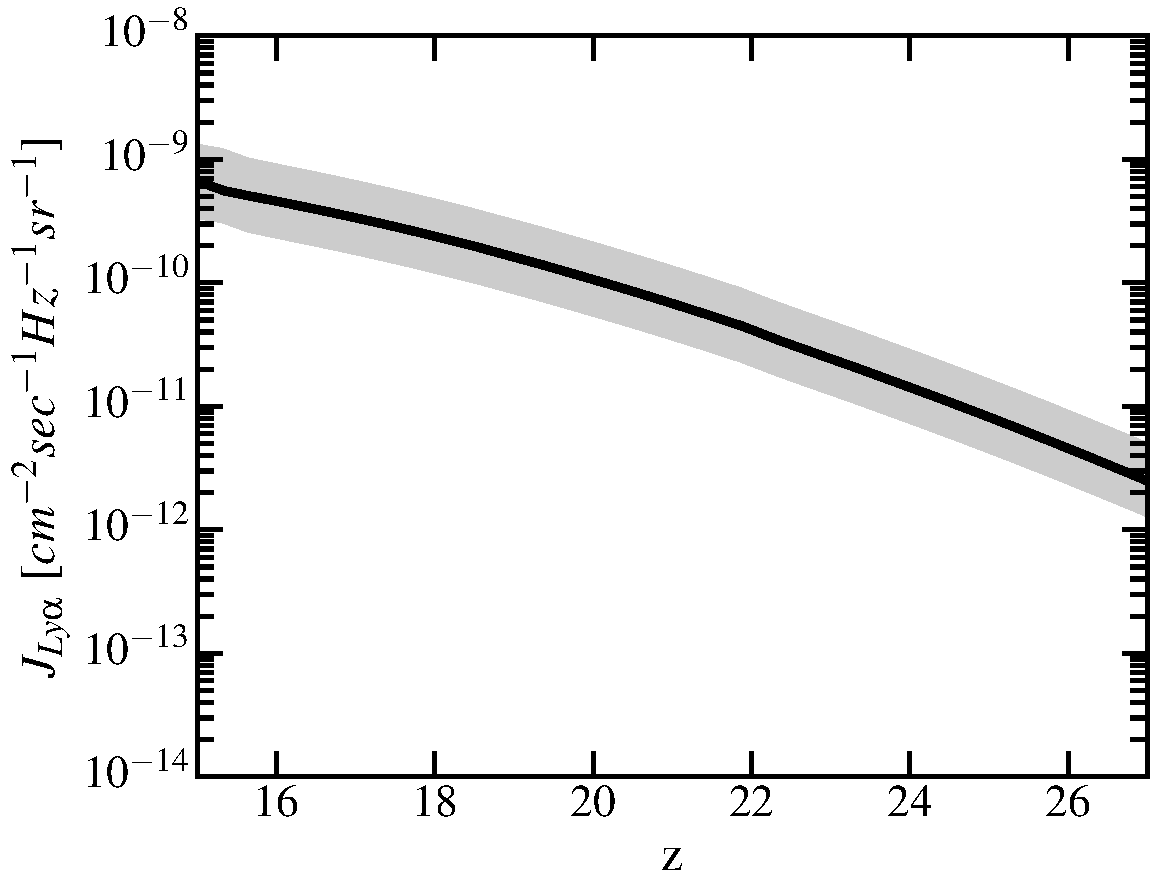
\includegraphics[width=.35\textwidth,keepaspectratio=true]{Jlya.pdf}
\caption{Cosmology.\label{fig:cosmo}}
\end{figure}
FFTT-like setup with a total collecting area of $(\Delta L)^2$=4 km$^2$, $\Omega_\text{survey}=1$sr, $t_\text{obs}$=2 year, assuming the array observed redshifts in the range $z\in [15,35]$. Figure \ref{fig:sigma_vs_deltas} shows how this sensitivity changes as a function of the maximum baseline.
\begin{figure}
\centering
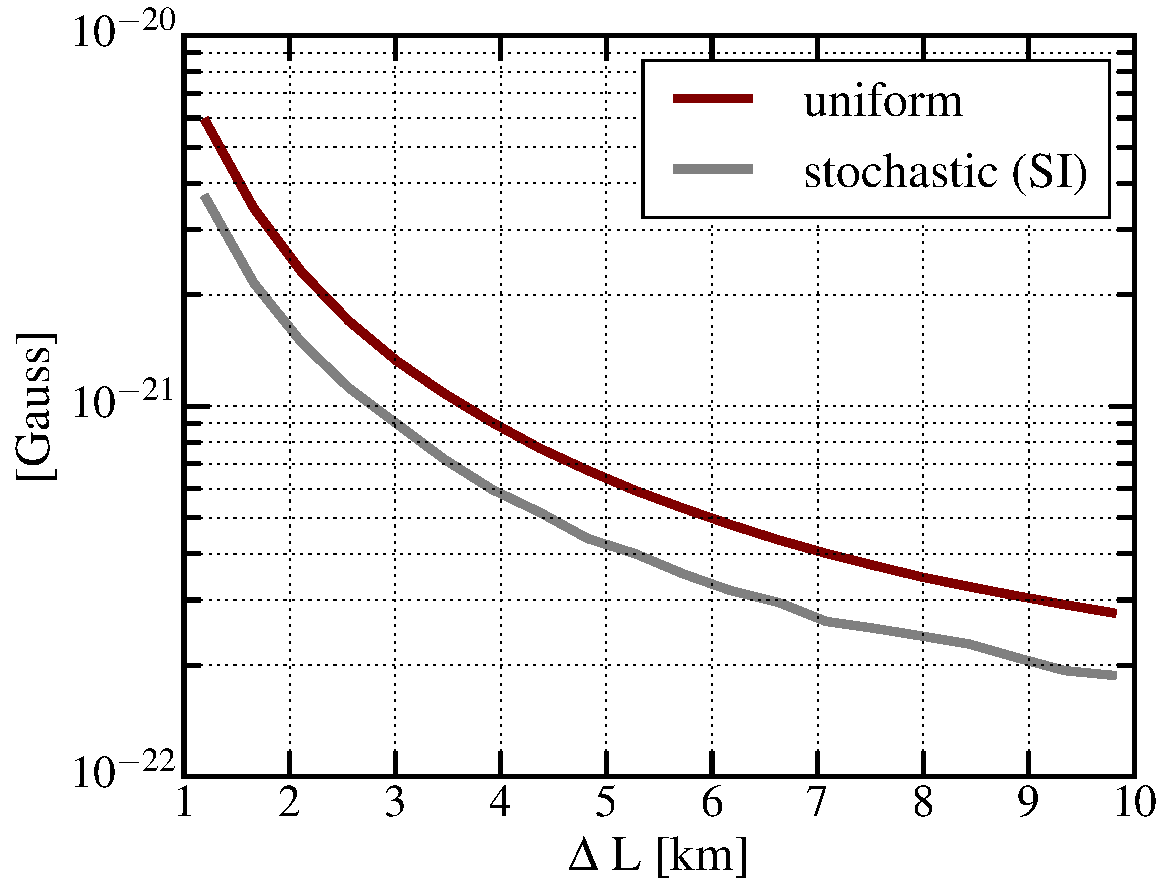
\includegraphics[width=.35\textwidth,keepaspectratio=true]{sigma_vs_deltas.pdf}
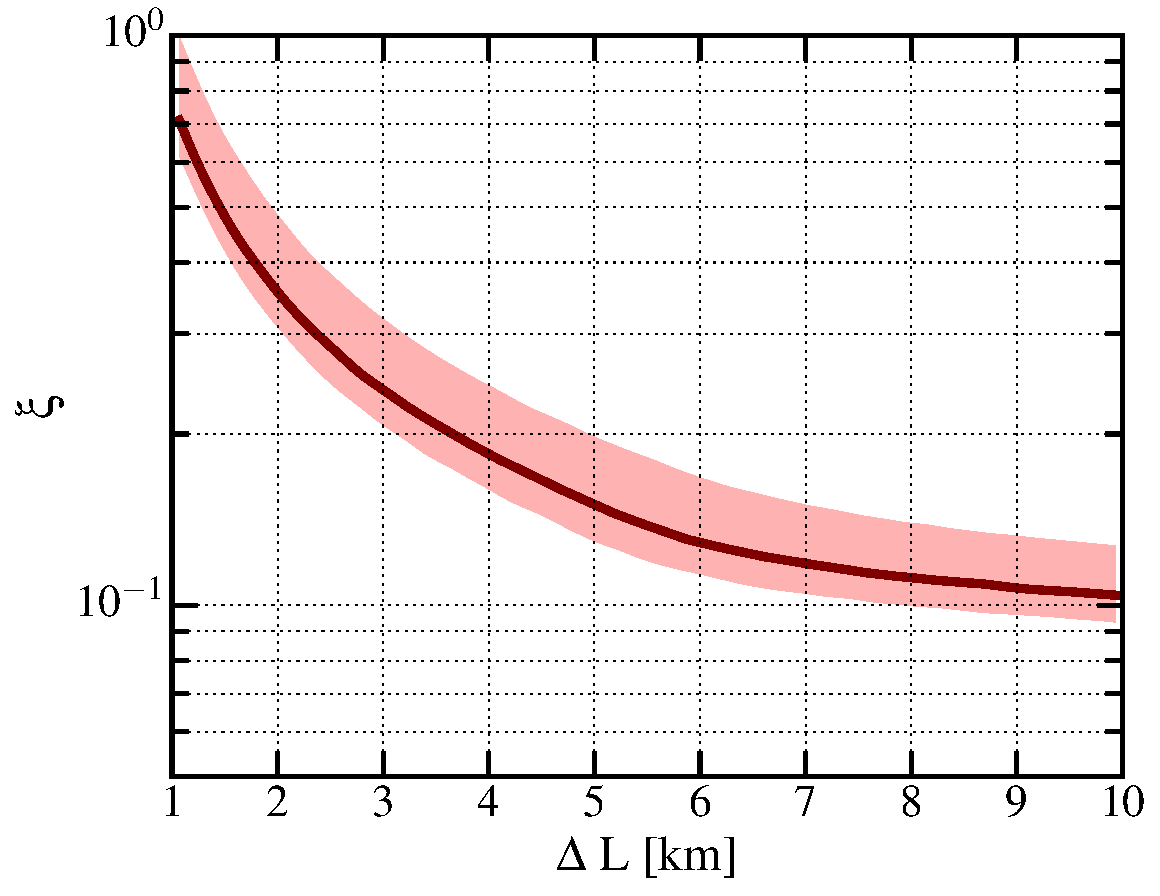
\includegraphics[width=.35\textwidth,keepaspectratio=true]{xi_vs_deltas.pdf}
\caption{FFTT sensitivity to detecting a uniform and stichastic magnetic field (upper panel; stochastic field is assumed to have a scale-independent power spectrum), and to distinguishing saturated case from no magnetic field (lower panel), as a function of maximum array baseline. Both are calculated for a survey size of 1 sr, for survey duration of 2 years.\label{fig:sigma_vs_deltas}}
\end{figure}
\begin{figure}
\centering
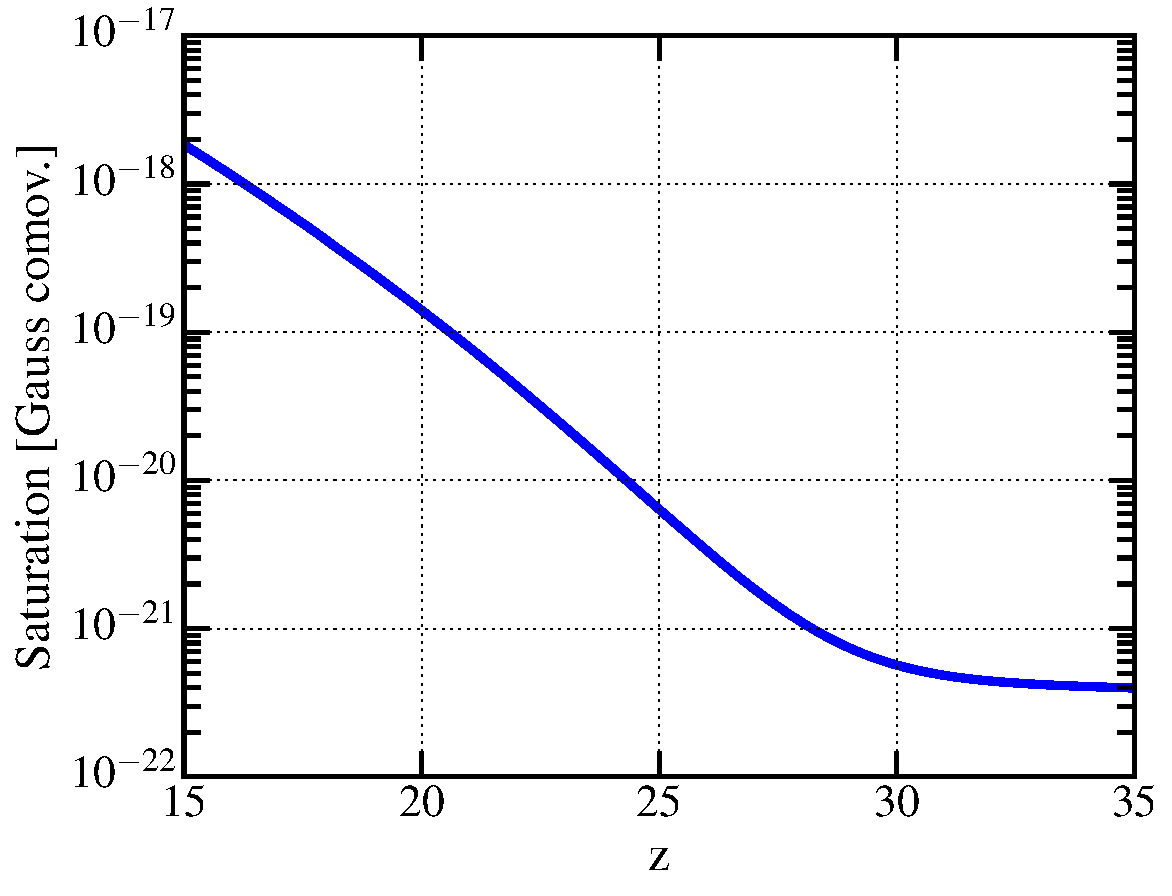
\includegraphics[width=.35\textwidth,keepaspectratio=true]{Bsaturation.pdf}
\caption{FFTT.\label{fig:Bsat}}
\end{figure}